\documentclass[11pt,a4paper]{article}

% Build with: pdflatex report.tex && pdflatex report.tex
% (the second pass resolves the table of contents and cross-references)

% ---------------------------------------------------------------------------
% Packages
% ---------------------------------------------------------------------------
\usepackage[utf8]{inputenc}
\usepackage[T1]{fontenc}
\usepackage{lmodern}
\usepackage[margin=2.5cm]{geometry}
\usepackage{amsmath,amssymb}
\usepackage{booktabs}
\usepackage{longtable}
\usepackage{array}
\usepackage{enumitem}
\usepackage{xcolor}
\usepackage{listings}
\usepackage{graphicx}
\usepackage{tikz}
\usetikzlibrary{positioning,arrows.meta}
\usepackage{setspace}
\usepackage{fancyhdr}
\usepackage{caption}
\usepackage{microtype}
\usepackage[colorlinks=true,linkcolor=blue!55!black,urlcolor=blue!55!black,citecolor=blue!55!black]{hyperref}

% ---------------------------------------------------------------------------
% Formatting
% ---------------------------------------------------------------------------
\onehalfspacing
\captionsetup{font=small,labelfont=bf}
\setlength{\parskip}{0.35em}
\setlength{\parindent}{0pt}

\pagestyle{fancy}
\fancyhf{}
\fancyhead[L]{\small Password Manager (POO)}
\fancyhead[R]{\small Technical Report}
\fancyfoot[C]{\thepage}
\renewcommand{\headrulewidth}{0.4pt}

\definecolor{codebg}{RGB}{248,248,248}
\definecolor{codekw}{RGB}{0,0,150}
\definecolor{codecomment}{RGB}{0,110,0}
\definecolor{codestring}{RGB}{150,0,0}
\definecolor{codegray}{RGB}{120,120,120}

\lstdefinestyle{java}{
  language=Java,
  basicstyle=\ttfamily\footnotesize,
  keywordstyle=\color{codekw}\bfseries,
  commentstyle=\color{codecomment}\itshape,
  stringstyle=\color{codestring},
  numbers=left,
  numberstyle=\tiny\color{codegray},
  numbersep=6pt,
  frame=single,
  rulecolor=\color{gray!40},
  backgroundcolor=\color{codebg},
  breaklines=true,
  showstringspaces=false,
  tabsize=2,
  captionpos=b
}

\lstdefinestyle{plaincode}{
  basicstyle=\ttfamily\footnotesize,
  frame=single,
  rulecolor=\color{gray!40},
  backgroundcolor=\color{codebg},
  breaklines=true,
  breakatwhitespace=false,
  showstringspaces=false,
  columns=fullflexible,
  captionpos=b
}

\lstdefinestyle{bash}{
  language=sh,
  basicstyle=\ttfamily\footnotesize,
  frame=single,
  rulecolor=\color{gray!40},
  backgroundcolor=\color{codebg},
  breaklines=true,
  showstringspaces=false,
  captionpos=b
}

\newcommand{\code}[1]{\texttt{#1}}

% ---------------------------------------------------------------------------
% Title page
% ---------------------------------------------------------------------------
\begin{document}

\begin{titlepage}
\centering
\vspace*{1.8cm}

{\Large\scshape University Name\par}
\vspace{0.4cm}
{\large Department of Computer Science\par}

\vspace{2.4cm}
{\Huge\bfseries A Secure Single-User\\[0.35cm] Password Manager in Java\par}

\vspace{0.9cm}
{\Large Design, Implementation and Cryptographic\\[0.2cm]
Verification of an Authenticated CLI Vault\par}

\vspace{1.4cm}
{\large Technical Report\par}

\vspace{1.8cm}
\begin{tabular}{rl}
\textbf{Course:}      & Object-Oriented Programming (POO)\\[2pt]
\textbf{Author:}      & Student Name\\[2pt]
\textbf{Student ID:}  & 000000000\\[2pt]
\textbf{Instructor:}  & Instructor Name\\[2pt]
\textbf{Date:}        & \today\\
\end{tabular}

\vfill
{\small Security indicators: IND1 (KEM), IND2 (Ed25519), IND3 (Schnorr ZKP)\par}
\end{titlepage}

% ---------------------------------------------------------------------------
% Abstract
% ---------------------------------------------------------------------------
\begin{abstract}
\noindent
This report documents the design, implementation and verification of a
single-user password manager written in Java 21. The application stores all
credentials in one authenticated, encrypted file and is operated from a
terminal. Confidentiality and integrity depend only on a master password and
standard cryptographic primitives: Argon2id for password-based key derivation,
AES-256-GCM for authenticated encryption, Ed25519 for digital signatures,
RSA-OAEP-SHA256 for key encapsulation (IND1) and an interactive Schnorr
zero-knowledge proof over RFC 3526 Group 14 for password authentication (IND3).
The master password derives a key-encryption key that protects the private keys,
while a random data-encryption key protects the credential database. The
Ed25519 signature is verified before any decryption is attempted, so tampering
is rejected early. Master-password rotation re-encrypts only the small key
material and re-wraps the data key; the credentials blob is preserved
byte-for-byte. The implementation is covered by 63 JUnit~5 tests, including
positive lifecycle tests and negative abuse scenarios, and three standalone
evidence programs demonstrate the indicators independently with reproducible
output. The report also states the threat model, trust assumptions, rejected
alternatives and residual limitations, and concludes that the design is suitable
as an academic prototype but not for production use without additional key
pinning, rollback protection and memory hardening.
\end{abstract}

\noindent\textbf{Keywords:} password manager, Argon2id, AES-GCM, Ed25519,
RSA-OAEP, Schnorr zero-knowledge proof, authenticated encryption, threat model.

\newpage
\tableofcontents
\newpage
\listoffigures
\listoftables
\newpage

% ===========================================================================
\section{Introduction}
% ===========================================================================

\subsection{Motivation}

Users accumulate dozens of online accounts, and reusing a single password across
them turns one breach into a cascade of compromises. Writing passwords down,
storing them in a spreadsheet or keeping them in a browser profile offers little
protection if the device is lost or the file is copied. Cloud password managers
solve part of the usability problem, but they move trust to a third party and
introduce a network attack surface.

A local password manager offers a different trade-off: the user keeps the vault
file and the master password, and no service provider is involved. The security
argument then reduces to the strength of the master password and the correctness
of the cryptographic construction. This project explores that trade-off in a
small, auditable Java codebase.

\subsection{Problem statement}

The project must provide a command-line, single-user password manager that:

\begin{enumerate}[label=\textbf{P\arabic*.},leftmargin=*]
  \item stores credentials confidentially in a single local file;
  \item detects any modification of that file before decrypting it;
  \item does not store a password-equivalent secret such as a password hash;
  \item separates the password-derived key from the key that protects the
        credential database;
  \item supports changing the master password without re-encrypting the whole
        credential database;
  \item runs as a normal Java application built with Maven and covered by
        automated tests.
\end{enumerate}

\subsection{Objectives}

\begin{itemize}[leftmargin=*]
  \item Design a clean domain model with a strict separation between the CLI,
        domain logic, persistence and cryptographic primitives.
  \item Implement the three indicators: a KEM (IND1), a digital signature scheme
        (IND2) and a zero-knowledge proof of knowledge (IND3).
  \item Provide an authenticated vault format and a signature-first loading
        procedure.
  \item Implement secure input, best-effort secret wiping and an atomic save.
  \item Verify the result with unit, integration, end-to-end and abuse tests, and
        with standalone evidence programs.
\end{itemize}

\subsection{Contributions}

The main contributions of the work are:

\begin{enumerate}[leftmargin=*]
  \item a layered architecture in which cryptographic primitives know nothing
        about the CLI or the vault file;
  \item a key hierarchy that separates the password-derived KEK from the random
        DEK, enabling cheap master-password rotation;
  \item an authenticated JSON vault whose Ed25519 signature is checked before
        any decryption;
  \item an interactive Schnorr authentication protocol that avoids storing a
        password hash;
  \item a test suite of 63 cases, including one-byte tampering and key
        substitution abuse scenarios;
  \item three reproducible evidence programs for IND1, IND2 and IND3.
\end{enumerate}

\subsection{Scope and non-goals}

The system is a single-user, offline, terminal application. It does not provide
multi-user access control, synchronisation, recovery, a graphical interface, a
browser extension or clipboard integration. It is an academic prototype, not a
production password manager; Section~\ref{sec:limitations} discusses the
remaining risks.

\subsection{Report structure}

Section~\ref{sec:background} introduces the cryptographic background.
Section~\ref{sec:requirements} states the requirements and the threat model.
Section~\ref{sec:design} presents the architecture and the main flows.
Section~\ref{sec:crypto} justifies the cryptographic choices and analyses the
composition. Section~\ref{sec:implementation} describes the implementation.
Section~\ref{sec:verification} reports the tests and evidence programs.
Section~\ref{sec:analysis} analyses security and residual risks.
Section~\ref{sec:discussion} discusses trade-offs, and
Section~\ref{sec:conclusions} concludes.

% ===========================================================================
\section{Background and related work}\label{sec:background}
% ===========================================================================

\subsection{Password managers}

Password managers are commonly classified as offline vaults, cloud-synchronised
vaults and browser-integrated managers. Offline vaults minimise the attack
surface but require the user to protect and back up the file. Cloud managers
improve availability and sharing but add a provider and a network to the trust
model. This project follows the offline model: one file, one user, one master
password.

\subsection{Password-based key derivation}

A password has low entropy compared with a cryptographic key, so a key-derivation
function (KDF) must slow down guessing. Argon2id~\cite{rfc9106} is the hybrid
variant of Argon2 recommended by RFC~9106. It combines a data-dependent first
half (resisting side-channel attacks) with a data-independent second half
(resisting time--memory trade-offs), and it is memory-hard: an attacker who wants
to test many passwords must allocate large amounts of memory per guess. This
project uses 64~MiB, three iterations, parallelism~1 and a 16-byte random salt.

Older alternatives include PBKDF2, bcrypt and scrypt. PBKDF2 is compute-hard but
not memory-hard; bcrypt truncates passwords at 72 bytes and has a fixed memory
footprint; scrypt is memory-hard but has a less side-channel-resistant design.
Argon2id is the modern default for new applications~\cite{nist80063b,owasp}.

\subsection{Authenticated encryption}

AES-GCM~\cite{nistgcm} is an authenticated encryption with associated data
(AEAD) mode. It provides confidentiality and integrity in one operation: a
128-bit authentication tag detects any modification of the ciphertext, the
nonce or the associated data. GCM requires a unique nonce per key; reusing a
nonce with the same key is catastrophic. This project generates a fresh random
96-bit nonce for every encryption and never reuses a nonce deliberately.

\subsection{Digital signatures}

Ed25519~\cite{rfc8032,bernstein2012} is a deterministic signature scheme built on
the twisted Edwards curve Curve25519. It offers roughly 128-bit security, small
32-byte public keys and 64-byte signatures, and avoids the nonce-reuse pitfalls
of ECDSA because the per-signature nonce is derived deterministically from the
private key and the message. The vault payload is signed with Ed25519 and the
signature is verified before decryption.

\subsection{Key encapsulation}

A key encapsulation mechanism (KEM) transports a symmetric key under a public
key. This project uses RSA-OAEP with SHA-256~\cite{rfc8017}: a random data
encryption key (DEK) is encrypted with the recipient's RSA public key and
recovered with the private key. OAEP provides a randomised, CCA-secure padding.
The older PKCS~\#1 v1.5 padding is vulnerable to Bleichenbacher-style
attacks~\cite{bleichenbacher1998} and is not used.

\subsection{Zero-knowledge proofs}

A zero-knowledge proof lets a prover convince a verifier that it knows a secret
without revealing it. The Schnorr protocol~\cite{schnorr1991} is a three-move
proof of knowledge of a discrete logarithm in a cyclic group. In this project
the secret is derived from the master password and the public verifier
$Y = g^x \bmod p$ is stored in the vault. Login runs the protocol interactively;
a wrong password produces a proof that fails verification, and no password hash
is stored.

\subsection{Threat modelling}

The design follows a simple asset--adversary--mitigation analysis. The main
adversary is an attacker with offline access to the vault file. The trusted
computing base is the local operating system, the JVM, the cryptographic
libraries and the terminal during an active session. The next section makes
these assumptions explicit.

% ===========================================================================
\section{Requirements and threat model}\label{sec:requirements}
% ===========================================================================

\subsection{Functional requirements}

\begin{table}[htbp]
\centering
\small
\begin{tabular}{@{}p{1.2cm}p{13.2cm}@{}}
\toprule
\textbf{ID} & \textbf{Requirement} \\
\midrule
FR1 & Register a new master user with a username and a master password. \\
FR2 & Unlock an existing vault with the master password. \\
FR3 & Add a credential (service, username, notes, password), optionally
      generating the password. \\
FR4 & List credentials without revealing their passwords. \\
FR5 & View the full details of a selected credential. \\
FR6 & Change the master password without re-encrypting the credential database. \\
FR7 & Save the vault, wipe session secrets and exit. \\
FR8 & Persist all changes across process restarts. \\
\bottomrule
\end{tabular}
\caption{Functional requirements.}
\label{tab:fr}
\end{table}

\subsection{Security requirements}

\begin{table}[htbp]
\centering
\small
\begin{tabular}{@{}p{1.2cm}p{13.2cm}@{}}
\toprule
\textbf{ID} & \textbf{Requirement} \\
\midrule
SR1 & Credentials must be confidential at rest. \\
SR2 & Any modification of the vault file must be detected before decryption. \\
SR3 & The vault must not contain a password-equivalent secret. \\
SR4 & The password-derived key and the credential-encryption key must be
      separated. \\
SR5 & The master password must be changeable without re-encrypting credentials. \\
SR6 & Secrets must be held in mutable buffers and wiped where practical. \\
SR7 & The implementation must reject weak or unsafe cryptographic modes
      (ECB, unauthenticated CBC, raw SHA-256 for passwords). \\
\bottomrule
\end{tabular}
\caption{Security requirements.}
\label{tab:sr}
\end{table}

\subsection{Protected assets}

\begin{table}[htbp]
\centering
\small
\begin{tabular}{@{}p{4.6cm}p{4.4cm}p{5.4cm}@{}}
\toprule
\textbf{Asset} & \textbf{Location} & \textbf{Protection} \\
\midrule
Master password & User memory / terminal & Never stored; derives KEK and ZKP secret \\
Credential passwords & \code{credentialsCiphertext} & AES-256-GCM under the DEK \\
Credential metadata & Same encrypted blob & AES-256-GCM \\
RSA private key & \code{kemPrivateKeyCiphertext} & AES-256-GCM under the KEK \\
Ed25519 private key & \code{signingPrivateKeyCiphertext} & AES-256-GCM under the KEK \\
Data-encryption key & \code{encapsulatedDek} & RSA-OAEP-SHA256 \\
Vault integrity & \code{signature} & Ed25519 over the payload \\
ZKP verifier $Y$ & \code{usuario.verifier} & Public; no password information \\
\bottomrule
\end{tabular}
\caption{Protected assets and their storage.}
\label{tab:assets}
\end{table}

\subsection{Adversaries and capabilities}

\begin{table}[htbp]
\centering
\small
\begin{tabular}{@{}p{3.5cm}p{5.2cm}p{5.7cm}@{}}
\toprule
\textbf{Adversary} & \textbf{Capability} & \textbf{Mitigation} \\
\midrule
Offline disk attacker & Reads, copies, modifies, replaces or deletes the vault & Argon2id slows guessing; Ed25519 rejects modifications; AES-GCM rejects ciphertext tampering; RSA-OAEP protects the DEK \\
Password guesser & Has the vault and tries candidate passwords offline & Argon2id with 64~MiB makes each guess expensive; no fast hash oracle is stored \\
File tamperer & Flips bytes in signature, ciphertext or metadata & Signature is verified before decryption; mismatch raises \code{SecurityException} \\
Impersonator & Runs the Schnorr protocol without the password & A proof made with the wrong secret fails verification \\
Wrong-key attacker & Tries to unwrap the DEK with an unrelated RSA key & RSA-OAEP unwrap fails \\
\bottomrule
\end{tabular}
\caption{Adversaries considered by the threat model.}
\label{tab:adversaries}
\end{table}

\subsection{Trust assumptions}

\begin{itemize}[leftmargin=*]
  \item \textbf{Trusted RAM during an active session.} While the vault is
        unlocked, the DEK, the private keys and the decrypted credentials exist
        in process memory. An attacker who can read memory, attach a debugger,
        inspect a core dump, swap or a hibernation image is out of scope.
  \item \textbf{Trusted platform.} The operating system, the JVM, the
        \code{SecureRandom} implementation, Bouncy Castle and Gson are assumed
        correct.
  \item \textbf{Trusted terminal.} \code{System.console().readPassword()}
        prevents echoing, but keyloggers and shoulder surfing are not
        prevented.
  \item \textbf{Sufficient master-password entropy.} Argon2id raises the cost of
        guessing but cannot rescue a trivial password.
  \item \textbf{No compromise during the session.} Malware with code execution
        can read memory or keystrokes and is out of scope.
\end{itemize}

\subsection{Out of scope}

The following are explicitly not protected: rollback to an older valid vault,
deletion of the vault, full-file substitution by a different self-consistent
vault, metadata leakage through file size, memory scraping, swap and
hibernation, clipboard leakage, and multi-user access control. These limitations
are revisited in Section~\ref{sec:limitations}.

\subsection{Indicator mapping}

\begin{table}[htbp]
\centering
\small
\begin{tabular}{@{}lll@{}}
\toprule
\textbf{Indicator} & \textbf{Primitive} & \textbf{Where it is used} \\
\midrule
IND1 & RSA-3072 OAEP-SHA256 & Wrapping and unwrapping the random DEK \\
IND2 & Ed25519 & Signing and verifying the vault payload \\
IND3 & Schnorr ZKP over RFC~3526 Group~14 & Master-password authentication \\
\bottomrule
\end{tabular}
\caption{Mapping between the course indicators and the implementation.}
\label{tab:indicators}
\end{table}

% ===========================================================================
\section{System design}\label{sec:design}
% ===========================================================================

\subsection{Layered architecture}

The code is organised in layers with dependencies pointing downward. The CLI
never touches ciphertext directly, and the cryptographic primitives never know
about the vault file.

\begin{figure}[htbp]
\centering
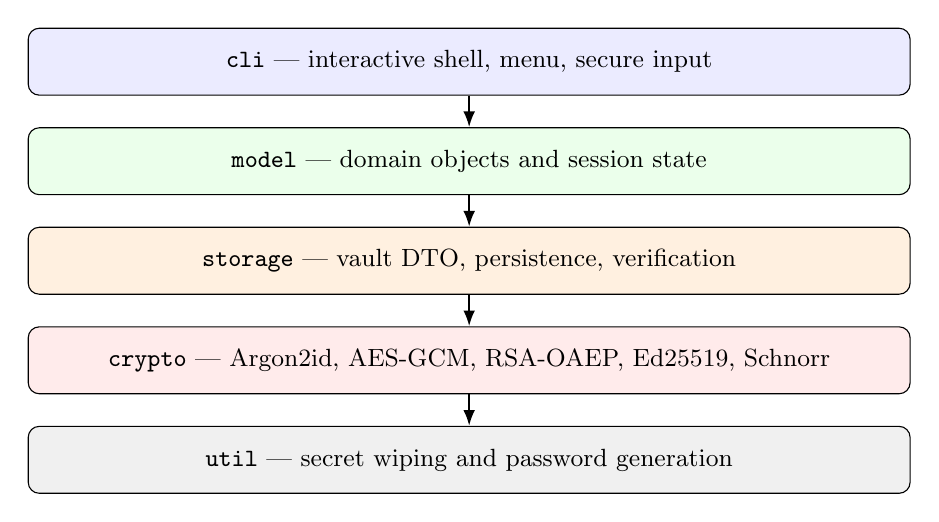
\begin{tikzpicture}[
  box/.style={draw, rounded corners, align=center, font=\small,
              minimum width=11.2cm, minimum height=0.85cm, inner sep=3pt},
  arr/.style={-{Latex[length=2mm]}, thick}
]
\node[box, fill=blue!8]   (cli)     {\code{cli} --- interactive shell, menu, secure input};
\node[box, fill=green!8, below=4mm of cli]   (model)   {\code{model} --- domain objects and session state};
\node[box, fill=orange!12, below=4mm of model] (storage) {\code{storage} --- vault DTO, persistence, verification};
\node[box, fill=red!8, below=4mm of storage]  (crypto)  {\code{crypto} --- Argon2id, AES-GCM, RSA-OAEP, Ed25519, Schnorr};
\node[box, fill=gray!12, below=4mm of crypto] (util)    {\code{util} --- secret wiping and password generation};
\draw[arr] (cli) -- (model);
\draw[arr] (model) -- (storage);
\draw[arr] (storage) -- (crypto);
\draw[arr] (crypto) -- (util);
\end{tikzpicture}
\caption{Layered architecture. Each layer depends only on the layers below it.}
\label{fig:layers}
\end{figure}

\subsection{Key hierarchy}

The design separates three secrets: the master password (never stored), the KEK
derived from it (transient) and the random DEK (stored only in encapsulated
form). Argon2id produces 64 bytes; the first 32 bytes are the KEK and the last
32 bytes seed the Schnorr secret. The separation prevents the ZKP secret from
being usable as an encryption key and vice versa.

\begin{figure}[htbp]
\centering
\resizebox{\textwidth}{!}{%
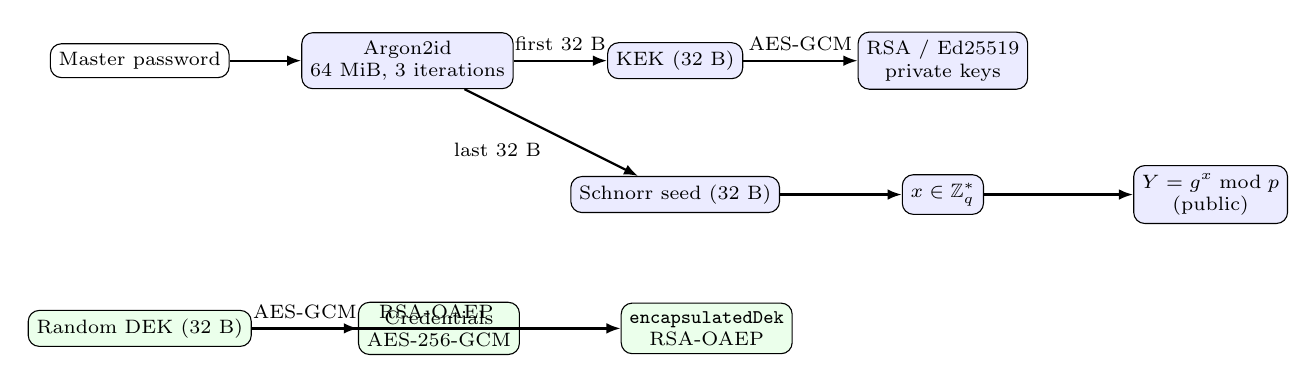
\begin{tikzpicture}[
  box/.style={draw, rounded corners, align=center, font=\scriptsize, inner sep=3pt},
  key/.style={box, fill=blue!8},
  data/.style={box, fill=green!8},
  arr/.style={-{Latex[length=1.8mm]}, thick}
]
\node[box] (pw) at (0,0) {Master password};
\node[key] (argon) at (3.4,0) {Argon2id\\64 MiB, 3 iterations};
\node[key] (kek) at (6.8,0) {KEK (32 B)};
\node[key] (priv) at (10.2,0) {RSA / Ed25519\\private keys};
\draw[arr] (pw) -- (argon);
\draw[arr] (argon) -- node[above,font=\scriptsize]{first 32 B} (kek);
\draw[arr] (kek) -- node[above,font=\scriptsize]{AES-GCM} (priv);

\node[key] (seed) at (6.8,-1.7) {Schnorr seed (32 B)};
\node[key] (x) at (10.2,-1.7) {$x \in \mathbb{Z}_q^{*}$};
\node[key] (y) at (13.6,-1.7) {$Y = g^{x} \bmod p$\\ (public)};
\draw[arr] (argon) -- node[below left,font=\scriptsize]{last 32 B} (seed);
\draw[arr] (seed) -- (x);
\draw[arr] (x) -- (y);

\node[data] (dek) at (0,-3.4) {Random DEK (32 B)};
\node[data] (blob) at (3.8,-3.4) {Credentials\\AES-256-GCM};
\node[data] (kem) at (7.2,-3.4) {\code{encapsulatedDek}\\RSA-OAEP};
\draw[arr] (dek) -- node[above,font=\scriptsize]{AES-GCM} (blob);
\draw[arr] (dek) -- node[above,font=\scriptsize]{RSA-OAEP} (kem);
\end{tikzpicture}%
}
\caption{Key hierarchy. The DEK is independent of the master password, so
rotation only replaces the password-derived material.}
\label{fig:keys}
\end{figure}

\subsection{Vault file format}

The vault is a UTF-8 JSON document with a signed payload. A Gson DTO
(\code{VaultFile}) holds the payload and the Base64-encoded Ed25519 signature.
The payload contains the master-user metadata, the encapsulated DEK and the
AES-GCM credentials blob.

\begin{lstlisting}[style=plaincode,caption={Abridged vault structure (boveda.json).},label={lst:vault}]
{
  "payload": {
    "usuario": {
      "salt": "<base64 16 bytes>",
      "verifier": "<base64 Y>",
      "kemPublicKey": "<base64 X.509 RSA>",
      "kemPrivateKeyIv": "<base64 12 bytes>",
      "kemPrivateKeyCiphertext": "<base64 AES-GCM>",
      "signingPublicKey": "<base64 X.509 Ed25519>",
      "signingPrivateKeyIv": "<base64 12 bytes>",
      "signingPrivateKeyCiphertext": "<base64 AES-GCM>",
      "nombreDeUsuario": "alice"
    },
    "encapsulatedDek": "<base64 RSA-OAEP>",
    "credentialsIv": "<base64 12 bytes>",
    "credentialsCiphertext": "<base64 AES-GCM>"
  },
  "signature": "<base64 Ed25519 over the canonical payload>"
}
\end{lstlisting}

The signature is computed over a compact, deterministic Gson serialization of
the payload (no pretty printing, HTML escaping disabled). The same serialization
is used at verification time, so field order and escaping cannot change the
signed bytes.

\subsection{Registration flow}

\begin{enumerate}[leftmargin=*]
  \item Generate a 16-byte random salt.
  \item Derive 64 bytes with Argon2id.
  \item Split the output: the first 32 bytes are the KEK, the last 32 bytes seed
        the Schnorr secret.
  \item Compute $Y = g^{x} \bmod p$ and store it as the public verifier.
  \item Generate an RSA-3072 key pair and an Ed25519 key pair.
  \item Encrypt both private keys with AES-256-GCM under the KEK.
  \item Generate a random 32-byte DEK and wrap it with RSA-OAEP-SHA256.
  \item Sign the canonical payload with Ed25519 and write the vault atomically.
\end{enumerate}

\subsection{Login flow}

\begin{enumerate}[leftmargin=*]
  \item Read \code{boveda.json} and verify the Ed25519 signature before asking
        for the password. A mismatch raises \code{SecurityException}.
  \item Prompt for the master password.
  \item Derive the master key and run the three-move Schnorr proof against the
        stored verifier.
  \item Only on success: derive the KEK, decrypt the private keys, decapsulate
        the DEK and decrypt the credential blob in memory.
\end{enumerate}

The order is deliberate: an attacker who tampers with the file cannot trigger
decryption or obtain a decryption oracle, because the signature check happens
first.

\subsection{Credential operations}

\begin{itemize}[leftmargin=*]
  \item \textbf{Add.} The CLI reads service, username, notes and an optional
        generated password. The new \code{Credential} is appended to the
        in-memory list and the vault is saved immediately, so an abrupt exit
        cannot lose it.
  \item \textbf{List.} Only service, username and notes are printed. Passwords
        are never included in the listing.
  \item \textbf{View.} The selected credential's password is copied to a
        temporary \code{char[]}, printed and wiped.
\end{itemize}

\subsection{Save and lock lifecycle}

Saving serializes the credential list, encrypts it with AES-256-GCM under the
DEK, wraps the DEK, signs the payload and writes the file atomically. Locking
zeroizes the DEK buffer, clears the in-memory credential passwords and drops
private-key references. The CLI calls \code{lock()} on exit and in its
\code{finally} block, so even an error path does not leave the session unlocked.

\subsection{Master-password rotation}

Rotation is the operation that motivates the KEK/DEK split:

\begin{enumerate}[leftmargin=*]
  \item Authenticate the current password with the ZKP.
  \item Derive a new KEK and a new Schnorr seed from the new password with a
        fresh salt.
  \item Re-encrypt the existing RSA and Ed25519 private keys under the new KEK.
  \item Recompute the verifier $Y$.
  \item Re-wrap the same DEK under the unchanged KEM public key.
  \item Re-sign the payload and reuse the existing \code{credentialsIv} and
        \code{credentialsCiphertext}.
\end{enumerate}

The old password stops working immediately, while the credentials blob is
preserved byte-for-byte. This is both a performance property and a correctness
property: rotation cannot corrupt or re-encrypt the large credential list.

\subsection{Class responsibilities}

\begin{table}[htbp]
\centering
\small
\begin{tabular}{@{}p{4.5cm}p{9.7cm}@{}}
\toprule
\textbf{Class} & \textbf{Responsibility} \\
\midrule
\code{cli.Main} & Menu, secure input, registration/login, rotation \\
\code{cli.PasswordManagerApp} & Registers the Bouncy Castle provider \\
\code{crypto.Argon2KDF} & Argon2id derivation with salt validation \\
\code{crypto.VaultCipher} & AES-256-GCM encrypt/decrypt and sealed data \\
\code{crypto.KeyEncapsulator} & RSA-3072 OAEP-SHA256 encapsulation (IND1) \\
\code{crypto.DigitalSigner} & Ed25519 key generation, sign and verify (IND2) \\
\code{crypto.SchnorrZKP} & Registration verifier and interactive proof (IND3) \\
\code{model.Credential} & Credential POJO with \code{char[]} password \\
\code{model.Usuario} & Base user type with public identity \\
\code{model.UsuarioMaestro} & Metadata, ZKP auth, encrypted private keys, rotation \\
\code{model.Gestor} & Singleton session: unlock, save, lock, rotation \\
\code{storage.VaultFile} & Gson DTO for payload and signature \\
\code{storage.PersistenciaBoveda} & Save/load, verify, decrypt, rewrap \\
\code{util.SecretWiper} & Best-effort zeroization \\
\code{util.GeneradorDeContrase\~nas} & Secure password generator \\
\code{evidencias.*} & Standalone IND1/IND2/IND3 demonstrations \\
\bottomrule
\end{tabular}
\caption{Main classes and their responsibilities.}
\label{tab:classes}
\end{table}

% ===========================================================================
\section{Cryptographic design and justification}\label{sec:crypto}
% ===========================================================================

\subsection{Argon2id}

Argon2id is used with a 16-byte random salt, 64~MiB of memory, three iterations
and parallelism~1. The 64-byte output is split into the KEK and the Schnorr
seed. The memory cost is the main defence against offline guessing: a GPU or
ASIC attacker must allocate 64~MiB per candidate password, which sharply reduces
parallelism compared with a fast hash.

The salt is stored in the vault and is not secret; its purpose is to prevent
precomputed tables and to ensure that two vaults with the same password derive
different keys.

\subsection{AES-256-GCM}

AES-256-GCM protects both the credentials blob and the private keys. Every
encryption uses a fresh 96-bit random nonce and produces a 128-bit tag. The
nonce is stored next to the ciphertext. Decryption fails with
\code{AEADBadTagException} if the ciphertext, nonce or tag is modified, or if the
wrong key is used.

The mode is used without associated data in this project; the Ed25519 signature
provides an additional, file-level integrity check. The two checks are
complementary: GCM protects the plaintext-to-ciphertext binding, while Ed25519
protects the whole payload, including metadata that is not encrypted.

\subsection{Ed25519}

Ed25519 signs the canonical payload. Signing is deterministic, so the same
payload and key always produce the same signature; this simplifies testing and
avoids nonce-reuse failures. Verification is performed before any decryption.
The signature covers the master-user metadata, the encapsulated DEK and the
credentials IV/ciphertext, so an attacker cannot change the KEM public key, the
verifier or the ciphertext without invalidating the signature.

\subsection{RSA-OAEP-SHA256 (IND1)}

The DEK is wrapped with RSA-3072 OAEP using SHA-256 as the digest and MGF1-SHA256
as the mask-generation function. Both hashes are pinned explicitly so that a
provider cannot silently fall back to SHA-1. OAEP is randomised: encapsulating
the same DEK twice produces different ciphertexts. Unwrapping with an unrelated
private key fails with a padding error.

RSA-3072 was chosen for compatibility with the JCA and for a comfortable margin
at the 128-bit security level. The KEM is used only to transport a 32-byte DEK;
it does not encrypt the credential database directly.

\subsection{Schnorr zero-knowledge proof (IND3)}

The proof runs in the prime-order subgroup of RFC~3526 Group~14~\cite{rfc3526}:
$p$ is a 2048-bit safe prime, $q = (p-1)/2$ is prime, and $g = 2$ generates the
order-$q$ subgroup. The prover knows $x \in [1, q-1]$ and the verifier knows
$Y = g^{x} \bmod p$.

\begin{enumerate}[leftmargin=*]
  \item The prover samples $r \gets \mathbb{Z}_q^{*}$ and sends
        $R = g^{r} \bmod p$.
  \item The verifier sends a random challenge $c \gets \mathbb{Z}_q^{*}$.
  \item The prover sends $s = (r + c\,x) \bmod q$.
  \item The verifier accepts iff $g^{s} \equiv R \cdot Y^{c} \pmod{p}$.
\end{enumerate}

The verifier also checks that $R$ and $Y$ lie in the order-$q$ subgroup. The
prover session is one-shot: a second response with the same commitment is
rejected, which prevents accidental nonce reuse. Because the protocol is
interactive and local, no Fiat--Shamir transform is needed.

The security intuition is standard: a prover without $x$ cannot answer a random
challenge except with negligible probability, and the transcript reveals no
information about $x$ beyond what can be simulated from $Y$ and $c$.

\subsection{Domain separation}

The same Argon2id invocation produces two 32-byte values with different
purposes. The KEK is used only with AES-GCM to encrypt private keys; the second
half is used only to derive the Schnorr secret. This avoids key reuse across
primitives and keeps the proof secret independent of the encryption key.

\subsection{Rejected alternatives}

\begin{table}[htbp]
\centering
\small
\begin{tabular}{@{}p{4.1cm}p{5.3cm}p{5.0cm}@{}}
\toprule
\textbf{Rejected option} & \textbf{Problem} & \textbf{Chosen instead} \\
\midrule
Raw or salted SHA-256 for passwords & Fast and GPU-friendly; enables massive offline guessing & Argon2id \\
PBKDF2 / bcrypt / scrypt & Weaker memory-hardness or side-channel profile; bcrypt truncates long passwords & Argon2id \\
AES-ECB & Deterministic, leaks plaintext patterns, no integrity & AES-256-GCM \\
AES-CBC without a MAC & Malleable; padding-oracle attacks & AES-256-GCM \\
AES-GCM with a reused nonce & Catastrophic key and tag recovery & Fresh random 96-bit nonce \\
RSA PKCS\#1 v1.5 & Bleichenbacher-style attacks & RSA-OAEP-SHA256 \\
ECDSA & Nonce reuse leaks the private key; fragile implementations & Ed25519 \\
Storing a password hash & Password-equivalent offline target & Schnorr verifier $Y$ \\
Plain JSON or Base64 & No confidentiality or integrity & AES-GCM + Ed25519 \\
\bottomrule
\end{tabular}
\caption{Rejected alternatives and the reasons for rejecting them.}
\label{tab:rejected}
\end{table}

\subsection{Informal security analysis}

\textbf{Confidentiality.} An attacker with the vault file must recover the DEK to
decrypt credentials, or the KEK to decrypt the private keys. Recovering the KEK
requires guessing the master password against Argon2id; recovering the DEK
requires breaking RSA-OAEP or AES-GCM. The credentials blob is encrypted under a
random 256-bit key, so it is not directly guessable.

\textbf{Integrity.} The Ed25519 signature covers the entire payload. A modified
payload fails verification before any AES-GCM operation. Even if the signature
were bypassed, GCM would reject a modified ciphertext or nonce. The two layers
protect different scopes: the signature protects metadata and structure, while
GCM protects the encrypted content.

\textbf{Authentication.} The Schnorr proof binds the login attempt to the secret
derived from the master password. A wrong password produces a different secret
and the proof fails. No password hash is stored, so a database leak does not
directly reveal a password-equivalent value.

\textbf{Rotation.} The new KEK and verifier are derived from the new password
with a fresh salt. The DEK and credentials blob are unchanged, so old
ciphertexts remain decryptable with the same DEK, while the old password can no
longer unlock the private keys or pass the proof.

% ===========================================================================
\section{Implementation}\label{sec:implementation}
% ===========================================================================

\subsection{Technology stack}

\begin{table}[htbp]
\centering
\small
\begin{tabular}{@{}lll@{}}
\toprule
\textbf{Component} & \textbf{Version} & \textbf{Role} \\
\midrule
Java & 21 & Language and runtime \\
Maven & 3.9+ & Build, tests and execution \\
Bouncy Castle (\code{bcprov-jdk18on}) & 1.78.1 & Argon2id and cryptographic support \\
Gson & 2.11.0 & JSON serialization \\
JUnit Jupiter & 5.11.0 & Automated tests \\
\bottomrule
\end{tabular}
\caption{Technology stack.}
\label{tab:stack}
\end{table}

Bouncy Castle~\cite{bc} supplies Argon2id and the provider bootstrap, while
Gson~\cite{gson} handles JSON serialization and deserialization.

\subsection{Project structure}

\begin{lstlisting}[style=plaincode,caption={Source tree.},label={lst:tree}]
src/main/java/
  cli/          Main, PasswordManagerApp
  crypto/       Argon2KDF, VaultCipher, KeyEncapsulator,
                DigitalSigner, SchnorrZKP
  model/        Credential, Usuario, UsuarioMaestro, Gestor
  storage/      VaultFile, PersistenciaBoveda
  util/         SecretWiper, GeneradorDeContrasenas
  evidencias/   EvidenciaKEM, EvidenciaFirma, EvidenciaZKP
src/test/java/  crypto, model, storage, security, cli, util
pom.xml
README.md
docs/report.tex
\end{lstlisting}

\subsection{Secure input and secret handling}

The CLI reads passwords with \code{System.console().readPassword()} when a
terminal is attached and falls back to a line-based \code{Scanner} otherwise.
Both paths return \code{char[]}, never \code{String}. The fallback is a
convenience for IDEs and pipes; it may echo input, so the documentation warns
users to run from a real terminal for daily use.

Secrets are held in mutable arrays and wiped with \code{SecretWiper} after use.
This is best-effort in Java: the garbage collector may copy arrays, and
\code{BigInteger} values cannot be zeroized. The code avoids obvious leaks such
as storing passwords in immutable strings or printing them from \code{toString()};
\code{Credential.toString()} prints \code{<protected>} instead of the password.

\subsection{Serialization and atomic persistence}

Gson serializes the vault DTO. A custom \code{TypeAdapter<char[]>} writes each
password character as a numeric UTF-16 code unit inside the encrypted blob, so
passwords never appear as JSON strings. The file is written to a temporary file
in the same directory and then moved over the destination with
\code{ATOMIC\_MOVE} when the filesystem supports it. On POSIX systems the
temporary file is created with owner-only permissions.

The signed serialization uses a separate Gson instance with pretty printing
disabled and HTML escaping disabled. This keeps the signed bytes stable and
independent of the display formatting.

\subsection{Exception model}

\begin{itemize}[leftmargin=*]
  \item \code{SecurityException} signals an authentication or integrity failure:
        a bad signature, a wrong master password or too many failed attempts.
  \item \code{GeneralSecurityException} signals a cryptographic operation
        failure, such as an OAEP unwrap error or an AEAD tag mismatch.
  \item \code{IOException} signals a filesystem failure.
  \item \code{IllegalArgumentException} signals invalid arguments, such as a
        wrong key size or an out-of-range Schnorr value.
\end{itemize}

The CLI catches these at the top level and reports a short message without a
stack trace, so a tampered file does not produce an unhandled exception.

\subsection{Representative code}

The following excerpts show the key operations. They are shortened for the
report; the full sources are in the repository.

\begin{lstlisting}[style=java,caption={Argon2id output split into KEK and Schnorr seed.},label={lst:argon}]
byte[] master = Argon2KDF.deriveKey(masterPassword, saltBytes, 64);
byte[] kek  = Arrays.copyOfRange(master, 0, 32);
byte[] seed = Arrays.copyOfRange(master, 32, 64);
BigInteger secret = SchnorrZKP.secretFromSeed(seed);
BigInteger verifier = SchnorrZKP.computeVerifier(secret);
\end{lstlisting}

\begin{lstlisting}[style=java,caption={AES-256-GCM with a fresh 96-bit nonce.},label={lst:gcm}]
byte[] iv = new byte[VaultCipher.IV_LENGTH_BYTES];
RANDOM.nextBytes(iv);
Cipher cipher = Cipher.getInstance("AES/GCM/NoPadding");
cipher.init(Cipher.ENCRYPT_MODE, key,
        new GCMParameterSpec(VaultCipher.TAG_LENGTH_BITS, iv));
byte[] ciphertext = cipher.doFinal(plaintext);
\end{lstlisting}

\begin{lstlisting}[style=java,caption={Schnorr verification.},label={lst:schnorr}]
BigInteger left  = G.modPow(response, P);
BigInteger right = commitment.multiply(verifier.modPow(challenge, P)).mod(P);
return MessageDigest.isEqual(left.toByteArray(), right.toByteArray());
\end{lstlisting}

\begin{lstlisting}[style=java,caption={Signature-first loading and DEK decapsulation.},label={lst:load}]
VaultFile file = PersistenciaBoveda.read(path);   // verifies Ed25519
byte[] dek = PersistenciaBoveda.decapsulateDek(file, kemPrivateKey);
List<Credential> credentials =
        PersistenciaBoveda.decryptCredentials(file, dek);
\end{lstlisting}

\subsection{Build and execution}

\begin{lstlisting}[style=bash,caption={Build, test and run commands.},label={lst:commands}]
mvn clean test
mvn exec:java
mvn exec:java -Dexec.args="/path/to/boveda.json"
mvn exec:java -Dexec.mainClass=evidencias.EvidenciaKEM
mvn exec:java -Dexec.mainClass=evidencias.EvidenciaFirma
mvn exec:java -Dexec.mainClass=evidencias.EvidenciaZKP
\end{lstlisting}

% ===========================================================================
\section{Verification and testing}\label{sec:verification}
% ===========================================================================

\subsection{Test strategy}

The suite combines four levels:

\begin{enumerate}[leftmargin=*]
  \item \textbf{Unit tests} for each primitive: deterministic KDF output, GCM
        round-trips and tamper rejection, KEM round-trips and wrong-key
        rejection, Ed25519 vectors, and Schnorr proof rejection cases.
  \item \textbf{Model and storage tests}: credential secret handling, ZKP
        authentication, session lock and DEK zeroization, vault save/reload,
        signature tampering and verify-before-decrypt.
  \item \textbf{End-to-end tests}: a full lifecycle from registration through
        save, reload, decryption and master-password rotation, plus scripted CLI
        sessions across restarts.
  \item \textbf{Abuse tests}: one-byte file tampering, one-byte AES-GCM
        tampering, ZKP impersonation and an unrelated KEM private key.
\end{enumerate}

\subsection{Test inventory}

\begin{table}[htbp]
\centering
\small
\begin{tabular}{@{}lrl@{}}
\toprule
\textbf{Package} & \textbf{Tests} & \textbf{Focus} \\
\midrule
\code{crypto}  & 29 & Argon2id, AES-GCM, RSA-OAEP, Ed25519, Schnorr \\
\code{model}   & 14 & Credential, UsuarioMaestro, Gestor \\
\code{storage} & 4  & Vault save/load, tampering, wrong DEK \\
\code{security}& 6  & End-to-end lifecycle and abuse scenarios \\
\code{cli}     & 6  & Scripted sessions and provider bootstrap \\
\code{util}    & 4  & Password generator \\
\midrule
\textbf{Total} & \textbf{63} & \\
\bottomrule
\end{tabular}
\caption{Test inventory.}
\label{tab:tests}
\end{table}

\subsection{Positive lifecycle test}

The end-to-end test performs the following steps in one flow:

\begin{enumerate}[leftmargin=*]
  \item create a master user and authenticate with the ZKP;
  \item unlock the private keys and generate a random DEK;
  \item save two credentials;
  \item reload the vault (Ed25519 verification);
  \item decapsulate the DEK and decrypt the credentials;
  \item rotate the master password;
  \item assert that the credentials IV and ciphertext are unchanged;
  \item assert that the old password fails and the new password succeeds;
  \item reload, decapsulate and decrypt again.
\end{enumerate}

The test also checks that the recovered DEK is identical before and after
rotation, which proves that rotation changes only the password-derived wrapping
material.

\subsection{Negative and abuse tests}

\begin{table}[htbp]
\centering
\small
\begin{tabular}{@{}p{4.3cm}p{5.0cm}p{5.0cm}@{}}
\toprule
\textbf{Scenario} & \textbf{Action} & \textbf{Expected result} \\
\midrule
Tampered file & Flip one byte of the Base64 signature in \code{boveda.json} & \code{SecurityException} from signature verification \\
Tampered vault ciphertext & Flip one byte of the stored credentials ciphertext & \code{SecurityException} before decryption \\
Tampered AES-GCM payload & Flip one byte of a GCM ciphertext & \code{AEADBadTagException} \\
ZKP impersonation & Authenticate with a wrong password; forge a proof with a different secret & Verification returns \code{false} \\
Wrong KEM key & Decapsulate the DEK with an unrelated RSA private key & \code{GeneralSecurityException} \\
\bottomrule
\end{tabular}
\caption{Abuse scenarios and expected results.}
\label{tab:abuse}
\end{table}

\subsection{Standalone evidence programs}

Three classes in \code{evidencias/} exercise the indicators without the CLI. They
use fixed demo material so that their printed output is reproducible, and they
end with \code{[RESULT] PASS}.

\begin{lstlisting}[style=bash,caption={Running the evidence programs.},label={lst:evidence}]
mvn exec:java -Dexec.mainClass=evidencias.EvidenciaKEM
mvn exec:java -Dexec.mainClass=evidencias.EvidenciaFirma
mvn exec:java -Dexec.mainClass=evidencias.EvidenciaZKP
\end{lstlisting}

\subsubsection{IND1 --- KEM}

\begin{lstlisting}[style=plaincode,caption={IND1 output (abridged).},label={lst:ind1}]
============================================================
 IND1 - KEM (RSA-OAEP-SHA256)
============================================================
[INPUT]  DEK (32 bytes): 000102...1c1d1e1f
[INPUT]  DEK SHA-256:    630dcd2966c4336691125448bbb25b4f...
[OUTPUT] KEM key pair: RSA / 3072-bit modulus
[OUTPUT] OAEP: SHA-256 digest, MGF1-SHA256
[OUTPUT] Encapsulated DEK length: 384 bytes
[OUTPUT] Recovered DEK: 000102...1c1d1e1f
[VERIFY] Recovered DEK equals input DEK: PASS
[VERIFY] Tampered encapsulation rejected: PASS
[VERIFY] Unrelated private key rejected: PASS

[RESULT] PASS
\end{lstlisting}

\subsubsection{IND2 --- Ed25519}

\begin{lstlisting}[style=plaincode,caption={IND2 output (abridged).},label={lst:ind2}]
============================================================
 IND2 - Digital Signature (Ed25519)
============================================================
[INPUT]  RFC 8032 TEST 1 seed (32 bytes): 9d61b19d...cae7f60
[OUTPUT] Derived public key (32 bytes): d75a9801...f707511a
[VERIFY] Derived public key matches RFC 8032: PASS
[OUTPUT] RFC 8032 signature (empty message): e5564300...8e7a100b
[VERIFY] Signature matches RFC 8032 vector: PASS
[INPUT]  Message: boveda.json|usuario=alice|credenciales=2
[OUTPUT] Signature (64 bytes): 4893009a...4572540e
[OUTPUT] Signature SHA-256: 1555bec5...3eea2e20
[VERIFY] Valid signature accepted: PASS
[VERIFY] One-byte signature tampering rejected: PASS
[VERIFY] Different message rejected: PASS

[RESULT] PASS
\end{lstlisting}

\subsubsection{IND3 --- Schnorr ZKP}

\begin{lstlisting}[style=plaincode,caption={IND3 output (abridged).},label={lst:ind3}]
============================================================
 IND3 - Schnorr Zero-Knowledge Proof (IND3)
============================================================
[INPUT]  Group: RFC 3526 Group 14 (p 2048 bits, q 2047 bits, g=2)
[INPUT]  Password (fixed demo value): "demo-master-password"
[INPUT]  Salt (16 bytes): 000102...0c0d0e0f
[OUTPUT] Secret x SHA-256:   dbb2b83a...f5f09625
[OUTPUT] Verifier Y SHA-256: e30c429a...aacc9c5a
[VERIFY] Verifier is in the order-q subgroup: PASS
[VERIFY] Registration is deterministic: PASS
[VERIFY] Valid proof accepted: PASS
[VERIFY] Impersonation with wrong password rejected: PASS
[VERIFY] Tampered response rejected: PASS

[RESULT] PASS
\end{lstlisting}

\subsection{Results}

\begin{table}[htbp]
\centering
\small
\begin{tabular}{@{}lr@{}}
\toprule
\textbf{Check} & \textbf{Result} \\
\midrule
Unit, integration, end-to-end and abuse tests & 63/63 pass \\
Evidence IND1 (KEM) & \code{[RESULT] PASS} \\
Evidence IND2 (Ed25519) & \code{[RESULT] PASS} \\
Evidence IND3 (Schnorr ZKP) & \code{[RESULT] PASS} \\
Repeated evidence runs produce identical output & Yes \\
\bottomrule
\end{tabular}
\caption{Verification results.}
\label{tab:results}
\end{table}

\subsection{Threats to validity}

The tests exercise the implemented code paths but do not constitute a formal
proof. There has been no independent cryptographic audit, no fuzzing campaign and
no constant-time analysis of the Java code. The evidence programs demonstrate
the primitives with fixed inputs; they do not prove the absence of
implementation flaws. These limitations are normal for a course project and are
stated explicitly rather than hidden.

% ===========================================================================
\section{Security analysis}\label{sec:analysis}
% ===========================================================================

\subsection{Attack surface}

The attack surface consists of: the vault file, the master password entry, the
CLI input parsing, the JSON deserialization path and the cryptographic
libraries. The application opens no network sockets and reads no external
configuration, so the file and the terminal are the main interfaces.

\subsection{Threats and mitigations}

\begin{table}[htbp]
\centering
\small
\begin{tabular}{@{}p{3.8cm}p{5.2cm}p{5.2cm}@{}}
\toprule
\textbf{Threat} & \textbf{Effect} & \textbf{Mitigation} \\
\midrule
Vault theft & Offline password guessing & Argon2id with 64~MiB; random salt; no fast hash oracle \\
Payload modification & Forged metadata or ciphertext & Ed25519 signature verified first \\
Ciphertext modification & Corrupted credentials & AES-GCM authentication tag \\
Wrong password & Unauthorised access & Schnorr proof fails \\
Wrong KEM key & DEK disclosure or decryption failure & RSA-OAEP unwrap fails \\
Replay of an old vault & Rollback & Not prevented (limitation) \\
Full-file substitution & Attacker-controlled vault & Not prevented without key pinning (limitation) \\
Memory scraping & Secret disclosure during session & Out of scope (trusted RAM) \\
\bottomrule
\end{tabular}
\caption{Threats and mitigations.}
\label{tab:threats}
\end{table}

\subsection{Residual risks and limitations}\label{sec:limitations}

\begin{itemize}[leftmargin=*]
  \item \textbf{Key substitution.} The signing public key is stored inside the
        signed payload. A complete replacement with a different, self-consistent
        vault is not detected unless the user pins the key or verifies a
        fingerprint out of band. A future version should store a fingerprint in
        a trusted location or use trust-on-first-use.
  \item \textbf{Rollback and deletion.} An attacker can restore an older valid
        vault or delete the file. A monotonic counter or an external anchor
        would be needed to detect rollback.
  \item \textbf{Metadata leakage.} The file size and ciphertext length reveal an
        approximate number and size of credentials. Padding could reduce this
        leakage at a cost in space.
  \item \textbf{Memory hygiene.} Java does not guarantee zeroization; arrays may
        be copied, and \code{BigInteger} values cannot be wiped. A native
        memory-safe implementation would be required for stronger guarantees.
  \item \textbf{No formal verification.} The protocol and implementation have
        not been machine-checked or audited.
  \item \textbf{Single user.} There is no access control beyond the master
        password, no recovery mechanism and no multi-device sync.
\end{itemize}

\subsection{Why the rejected alternatives matter}

Using raw SHA-256 for the master password would turn the vault into a
high-speed offline guessing target. AES-ECB would reveal equality patterns
between credentials and provide no integrity. CBC without a MAC would be
malleable and vulnerable to padding oracles. RSA PKCS\#1 v1.5 would expose the
DEK wrapping to Bleichenbacher-style attacks. ECDSA would introduce nonce-reuse
risk. The chosen primitives avoid these failure modes and are widely reviewed.

% ===========================================================================
\section{Discussion}\label{sec:discussion}
% ===========================================================================

\subsection{Design trade-offs}

\begin{itemize}[leftmargin=*]
  \item \textbf{Argon2id memory vs. responsiveness.} 64~MiB and three
        iterations make login noticeably slower than a fast hash, but that is
        the point: the cost is paid by the attacker as well. The parameters can
        be tuned if the target device is memory-constrained.
  \item \textbf{ZKP vs. password hash.} The Schnorr verifier avoids storing a
        password-equivalent value, but it does not eliminate offline guessing:
        an attacker can still test a candidate password by deriving the secret
        and checking the verifier. Argon2id is what makes that expensive.
  \item \textbf{RSA vs. elliptic-curve KEM.} RSA-3072 is widely supported and
        simple to use with the JCA, but its keys and ciphertexts are large. An
        ECIES or X25519-based KEM would be more compact; RSA was chosen for
        clarity and compatibility.
  \item \textbf{Interactive ZKP vs. non-interactive proof.} The local CLI can
        run the three-move protocol directly. A network or stateless setting
        would require Fiat--Shamir and a carefully designed transcript.
  \item \textbf{Single file vs. database.} A single JSON file is easy to back
        up and inspect, but it does not scale to large vaults and does not
        support concurrent writers.
\end{itemize}

\subsection{Lessons learned}

\begin{itemize}[leftmargin=*]
  \item Separating the KEK from the DEK makes rotation cheap and keeps the
        credential blob stable; this was the most useful design decision.
  \item Verifying the signature before decryption simplifies the error model:
        tampering is rejected as an integrity failure, not as a decryption
        failure.
  \item Java's immutable strings are a poor fit for secrets. Using
        \code{char[]} and wiping aggressively is better, but the language still
        limits how far memory hygiene can go.
  \item Reproducible evidence is valuable: fixed inputs and a known-answer
        vector make the cryptographic behaviour easy to demonstrate and grade.
  \item Tests are most convincing when they include abuse cases, not only happy
        paths.
\end{itemize}

\subsection{Comparison with alternatives}

A cloud password manager offers synchronisation, sharing and recovery, but adds
a provider and a network to the trust model. A plain encrypted file offers
confidentiality but usually lacks integrity, rotation and a structured format.
This project occupies a middle ground: a local file with authenticated
encryption, a signature, a ZKP login and a clean rotation path, at the cost of
manual backup and no multi-device support.

% ===========================================================================
\section{Conclusions and future work}\label{sec:conclusions}
% ===========================================================================

\subsection{Conclusions}

The project delivers a working, tested, single-user password manager that
combines five cryptographic mechanisms in a coherent design. Argon2id derives
the KEK and the Schnorr secret from the master password; AES-256-GCM protects
the credentials and private keys; Ed25519 authenticates the vault payload;
RSA-OAEP-SHA256 encapsulates the DEK (IND1); and the Schnorr proof authenticates
the user without storing a password hash (IND3). The signature-first loading
order, the KEK/DEK separation and the cheap master-password rotation are the
central design ideas.

The implementation is covered by 63 automated tests, including one-byte
tampering, ZKP impersonation and wrong-key decapsulation, and by three
standalone evidence programs with reproducible output. The design meets the
stated functional and security requirements within its threat model. It is an
academic prototype, not a production password manager: key pinning, rollback
protection and memory hardening remain future work.

\subsection{Future work}

\begin{enumerate}[leftmargin=*]
  \item \textbf{Key pinning / TOFU.} Store or display a signing-key fingerprint
        so a full-file substitution is detectable.
  \item \textbf{Rollback protection.} Add a monotonic counter or an external
        anchor to detect restored old vaults.
  \item \textbf{Memory hardening.} Explore native memory, guarded buffers or a
        dedicated secret-handling library; document the limits of Java.
  \item \textbf{Stronger authentication.} Add a second factor (FIDO2/WebAuthn) or
        a hardware-backed key store.
  \item \textbf{Formal analysis.} Model the protocol and the key hierarchy in a
        proof assistant or apply a symbolic protocol verifier.
  \item \textbf{Usability.} Add clipboard integration with automatic clearing,
        a search command, import/export and a graphical front end.
  \item \textbf{Packaging.} Produce a fat jar or a native image and add
        integration tests for the packaged artifact.
  \item \textbf{Audit and fuzzing.} Run a fuzzing campaign on the JSON parser and
        the CLI input paths, and commission an independent review.
\end{enumerate}

% ===========================================================================
% References
% ===========================================================================
\begin{thebibliography}{99}

\bibitem{rfc9106}
A.~Biryukov, D.~Dinu, D.~Khovratovich, and S.~Josefsson,
``Argon2 Memory-Hard Function for Password Hashing and Proof-of-Work
Applications,'' RFC~9106, IETF, 2021.

\bibitem{rfc8032}
S.~Josefsson and I.~Liusvaara,
``Edwards-Curve Digital Signature Algorithm (EdDSA),'' RFC~8032, IETF, 2017.

\bibitem{rfc8017}
K.~Moriarty, B.~Kaliski, J.~Jonsson, and A.~Rusch,
``PKCS \#1: RSA Cryptography Specifications Version 2.2,'' RFC~8017, IETF, 2016.

\bibitem{nistgcm}
M.~Dworkin,
``Recommendation for Block Cipher Modes of Operation: Galois/Counter Mode (GCM)
and GMAC,'' NIST Special Publication 800-38D, 2007.

\bibitem{rfc3526}
T.~Kivinen and M.~Kojo,
``More Modular Exponential (MODP) Diffie-Hellman groups for Internet Key
Exchange (IKE),'' RFC~3526, IETF, 2003.

\bibitem{schnorr1991}
C.~P. Schnorr,
``Efficient Signature Generation by Smart Cards,''
\emph{Journal of Cryptology}, vol.~4, no.~3, pp.~161--174, 1991.

\bibitem{bernstein2012}
D.~J. Bernstein, N.~Duif, T.~Lange, P.~Schwabe, and B.-Y. Yang,
``High-Speed High-Security Signatures,''
\emph{Journal of Cryptographic Engineering}, vol.~2, no.~2, pp.~77--89, 2012.

\bibitem{bleichenbacher1998}
D.~Bleichenbacher,
``Chosen Ciphertext Attacks Against Protocols Based on the RSA Encryption
Standard PKCS \#1,'' in \emph{Advances in Cryptology -- CRYPTO~'98},
LNCS~1462, pp.~1--12, 1998.

\bibitem{nist80063b}
P.~A. Grassi, M.~E. Garcia, and J.~L. Fenton,
``Digital Identity Guidelines: Authentication and Lifecycle Management,''
NIST Special Publication 800-63B, 2017.

\bibitem{owasp}
OWASP Foundation,
``Password Storage Cheat Sheet,'' OWASP Cheat Sheet Series, 2023.

\bibitem{bc}
The Legion of the Bouncy Castle,
``Bouncy Castle Cryptography Library,'' \url{https://www.bouncycastle.org/}.

\bibitem{gson}
Google,
``Gson: A Java serialization/deserialization library,'' 
\url{https://github.com/google/gson}.

\end{thebibliography}

% ===========================================================================
% Appendices
% ===========================================================================
\newpage
\appendix

\section{CLI transcript}

\begin{lstlisting}[style=plaincode,caption={Registration, add, save and reload (abridged).},label={lst:transcript}]
No vault found. First-run registration.
Username: alice
Master password: ********
Confirm master password: ********
Vault created: /home/alice/boveda.json

=== Password Manager ===
1. Add credential
2. List credentials
3. View credential details
4. Change master password
5. Save, wipe memory and exit
0. Exit without saving
Option: 1
Service: github
Username/email: alice
Notes: work account
Generate a password? (y/N): n
Password: ********
Credential added and saved.

=== Password Manager ===
...
Option: 5
Saved. Exiting.

$ mvn exec:java -Dexec.args="boveda.json"
Master password: ********
Vault unlocked.

=== Password Manager ===
...
Option: 2
1. github | alice | work account

=== Password Manager ===
...
Option: 0
Exiting without saving.
\end{lstlisting}

\section{Test commands and results}

\begin{lstlisting}[style=bash,caption={Full test run.},label={lst:testrun}]
$ mvn clean test
...
[INFO] Tests run: 63, Failures: 0, Errors: 0, Skipped: 0
[INFO] BUILD SUCCESS
\end{lstlisting}

\begin{lstlisting}[style=bash,caption={Evidence programs.},label={lst:evidencerun}]
$ mvn exec:java -Dexec.mainClass=evidencias.EvidenciaKEM
...
[RESULT] PASS

$ mvn exec:java -Dexec.mainClass=evidencias.EvidenciaFirma
...
[RESULT] PASS

$ mvn exec:java -Dexec.mainClass=evidencias.EvidenciaZKP
...
[RESULT] PASS
\end{lstlisting}

\section{Glossary}

\begin{description}[leftmargin=*,style=nextline]
  \item[AEAD] Authenticated Encryption with Associated Data.
  \item[DEK] Data-Encryption Key; the random key that protects credentials.
  \item[GCM] Galois/Counter Mode, an AEAD mode for block ciphers.
  \item[IND1/IND2/IND3] The course security indicators: KEM, signatures and ZKP.
  \item[KDF] Key-Derivation Function.
  \item[KEK] Key-Encryption Key; derived from the master password.
  \item[KEM] Key-Encapsulation Mechanism.
  \item[OAEP] Optimal Asymmetric Encryption Padding.
  \item[TOFU] Trust On First Use.
  \item[ZKP] Zero-Knowledge Proof.
\end{description}

\end{document}
